\documentclass[12pt,a4paper]{article}
\usepackage[utf8]{inputenc}
\usepackage{graphicx}   % Para insertar gráficos
\usepackage{geometry}   % Para márgenes
\geometry{top=2.5cm, bottom=2.5cm, left=2.5cm, right=2.5cm}
\usepackage{setspace}   % Para controlar espacio entre líneas
\usepackage{lipsum}     % Solo para texto de ejemplo

% ---------------- Caratula ----------------
\begin{document}
\begin{titlepage}
    \centering
    \vspace*{2cm}
    
    {\Huge \textbf{Alix Partners: La Casa de Asterión}}\\[0.5cm]
    {\Large Predicción de demanda y optimización de precios}\\[1.5cm]
    
    {\Large Integrantes:}\\
    \vspace{0.5cm}
    Juan Cruz Mendoza\\
    Joaquín Miceli\\[1cm]
    
    {\Large 2025}\\[2cm]

\end{titlepage}

% ---------------- Contenido ----------------
\tableofcontents
\newpage

\section{Introducción}

En esta competencia, nos fue dado el siguiente desafío: un negocio de ventas minoristas, llamado "La Casa de Asterión", ha sufrido una reducción de ganancias 
en el último tiempo, y necesita mejorar su estrategia de precios. La empresa ha proporcionado los siguientes datos: las transacciones de ventas de los últimos 3 años, 
especificando las tiendas, los productos vendidos y sus precios. Además, también contamos con datos sobre las tiendas, como su ubicación, y sobre los productos, como su 
categoría y marca. 

\vspace{0.2cm}

Entonces, valiéndonos de toda esta información, nuestro objetivo es contruir un modelo capaz de predecir la demanda diaria de los prodcutos de la próxima semana a 
partir del precio y otras variables, y con el mismo, optimizar los precios para maximizar las ganancias.

\vspace{0.2cm}

Dado que desconocemos si el cliente tiene conocimientos técnicos acerca de programación y desarrollo de modelos de AI, 
hemos decidido dividir este informe en dos secciones: por un lado, un análisis económico, el cual no necesita conocimientos técnicos para ser entendido, 
donde analizamos realizamos un análisis de datos básico y exponemos una estrategia de precios que, según las predicciones hechas, debería aumentar las ganancias; 
y por otro lado, realizamos un análisis técnico, en donde detallamos el preprocesamiento de datos, la construcción y entrenamiento del modelo predictivo 
y la metodología de optimización de precios.


\section{Análisis Económico}

En primer lugar, nos preguntamos por qué se ha producido una caída de las ganancias y qué tan grave es. Para esto, se puede observar 
en el siguiente gráfico cómo fue evolucionando la ganancia total de la empresa a lo largo del tiempo, y cómo la misma ha ido disminuyendo de a poco 
en el transcurso del tiempo.

\begin{center}
    \makebox[\textwidth][c]{%
        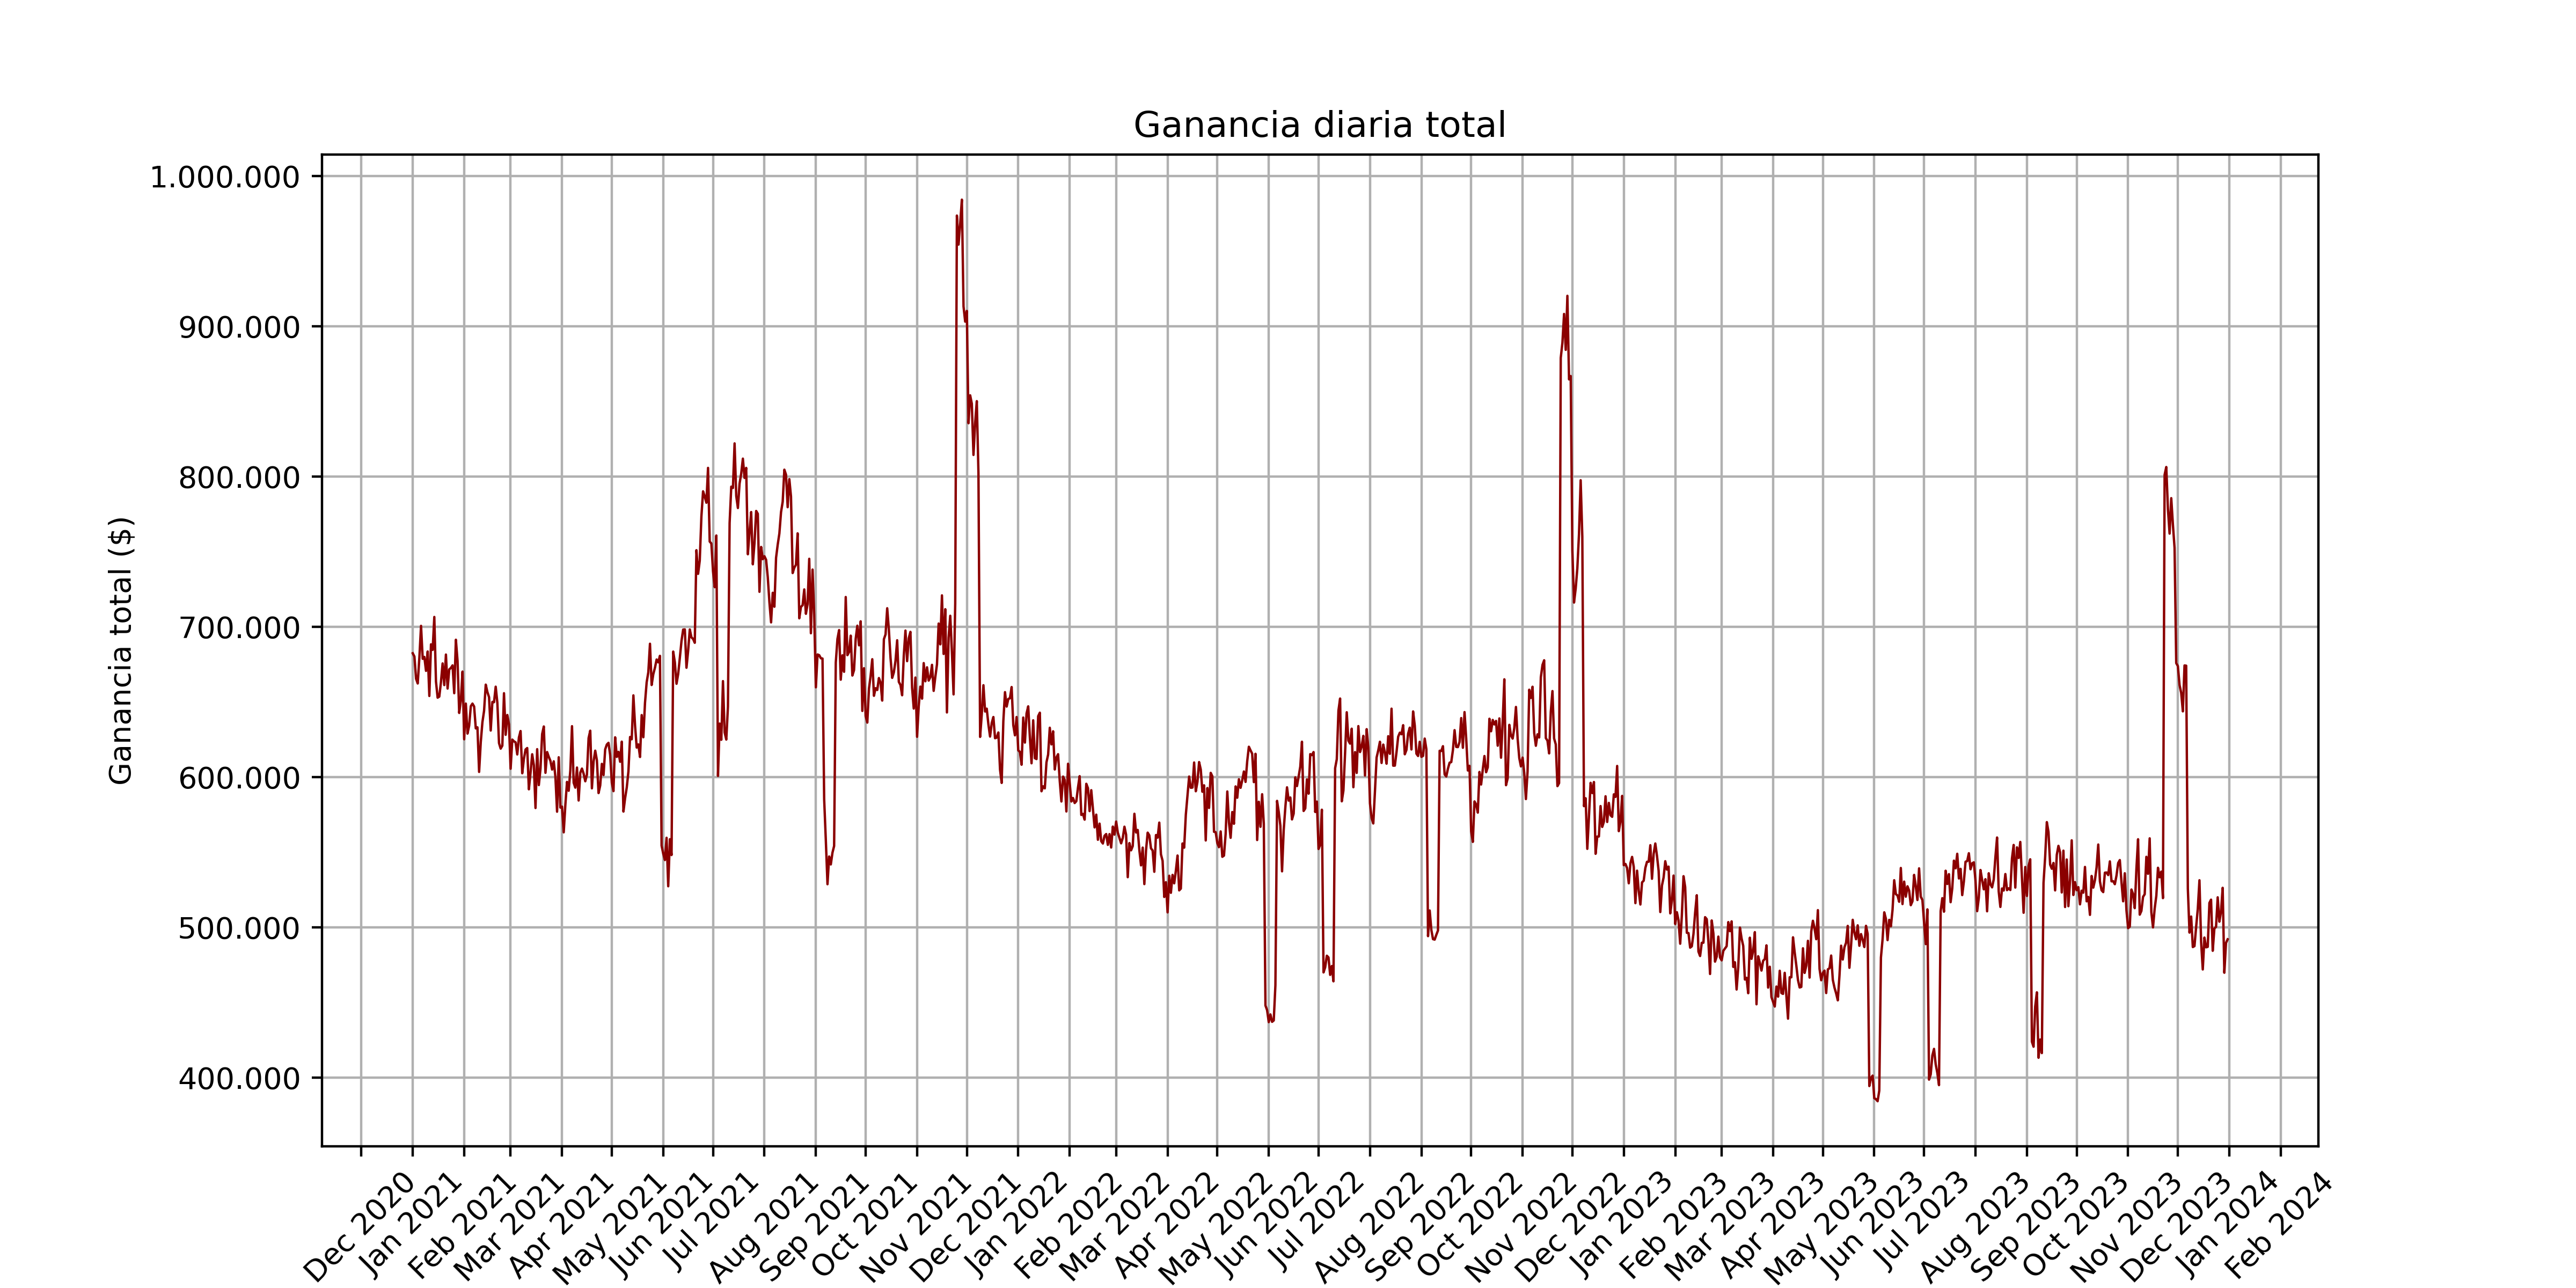
\includegraphics[width=1.2\textwidth]{graficos/ganancia_diaria_total.png}%
    }
\end{center}

En concreto, con respecto al primer año, las ganancias totales se han reducido un 11.3\% en el segundo año y un 23.7\% en el tercer año, 
lo cual puede resultar preocupante.

\vspace{0.2cm}

Este fenómeno puede deberse en gran parte a la reducción de la demanda total, que ha disminuído 10\% el primer año y un 21.2\% en el segundo año. 
Esto se puede apreciar en el siguiente gráfico, además de cómo varía la demanda según la categoría de los productos:

\begin{center}
    \makebox[\textwidth][c]{%
        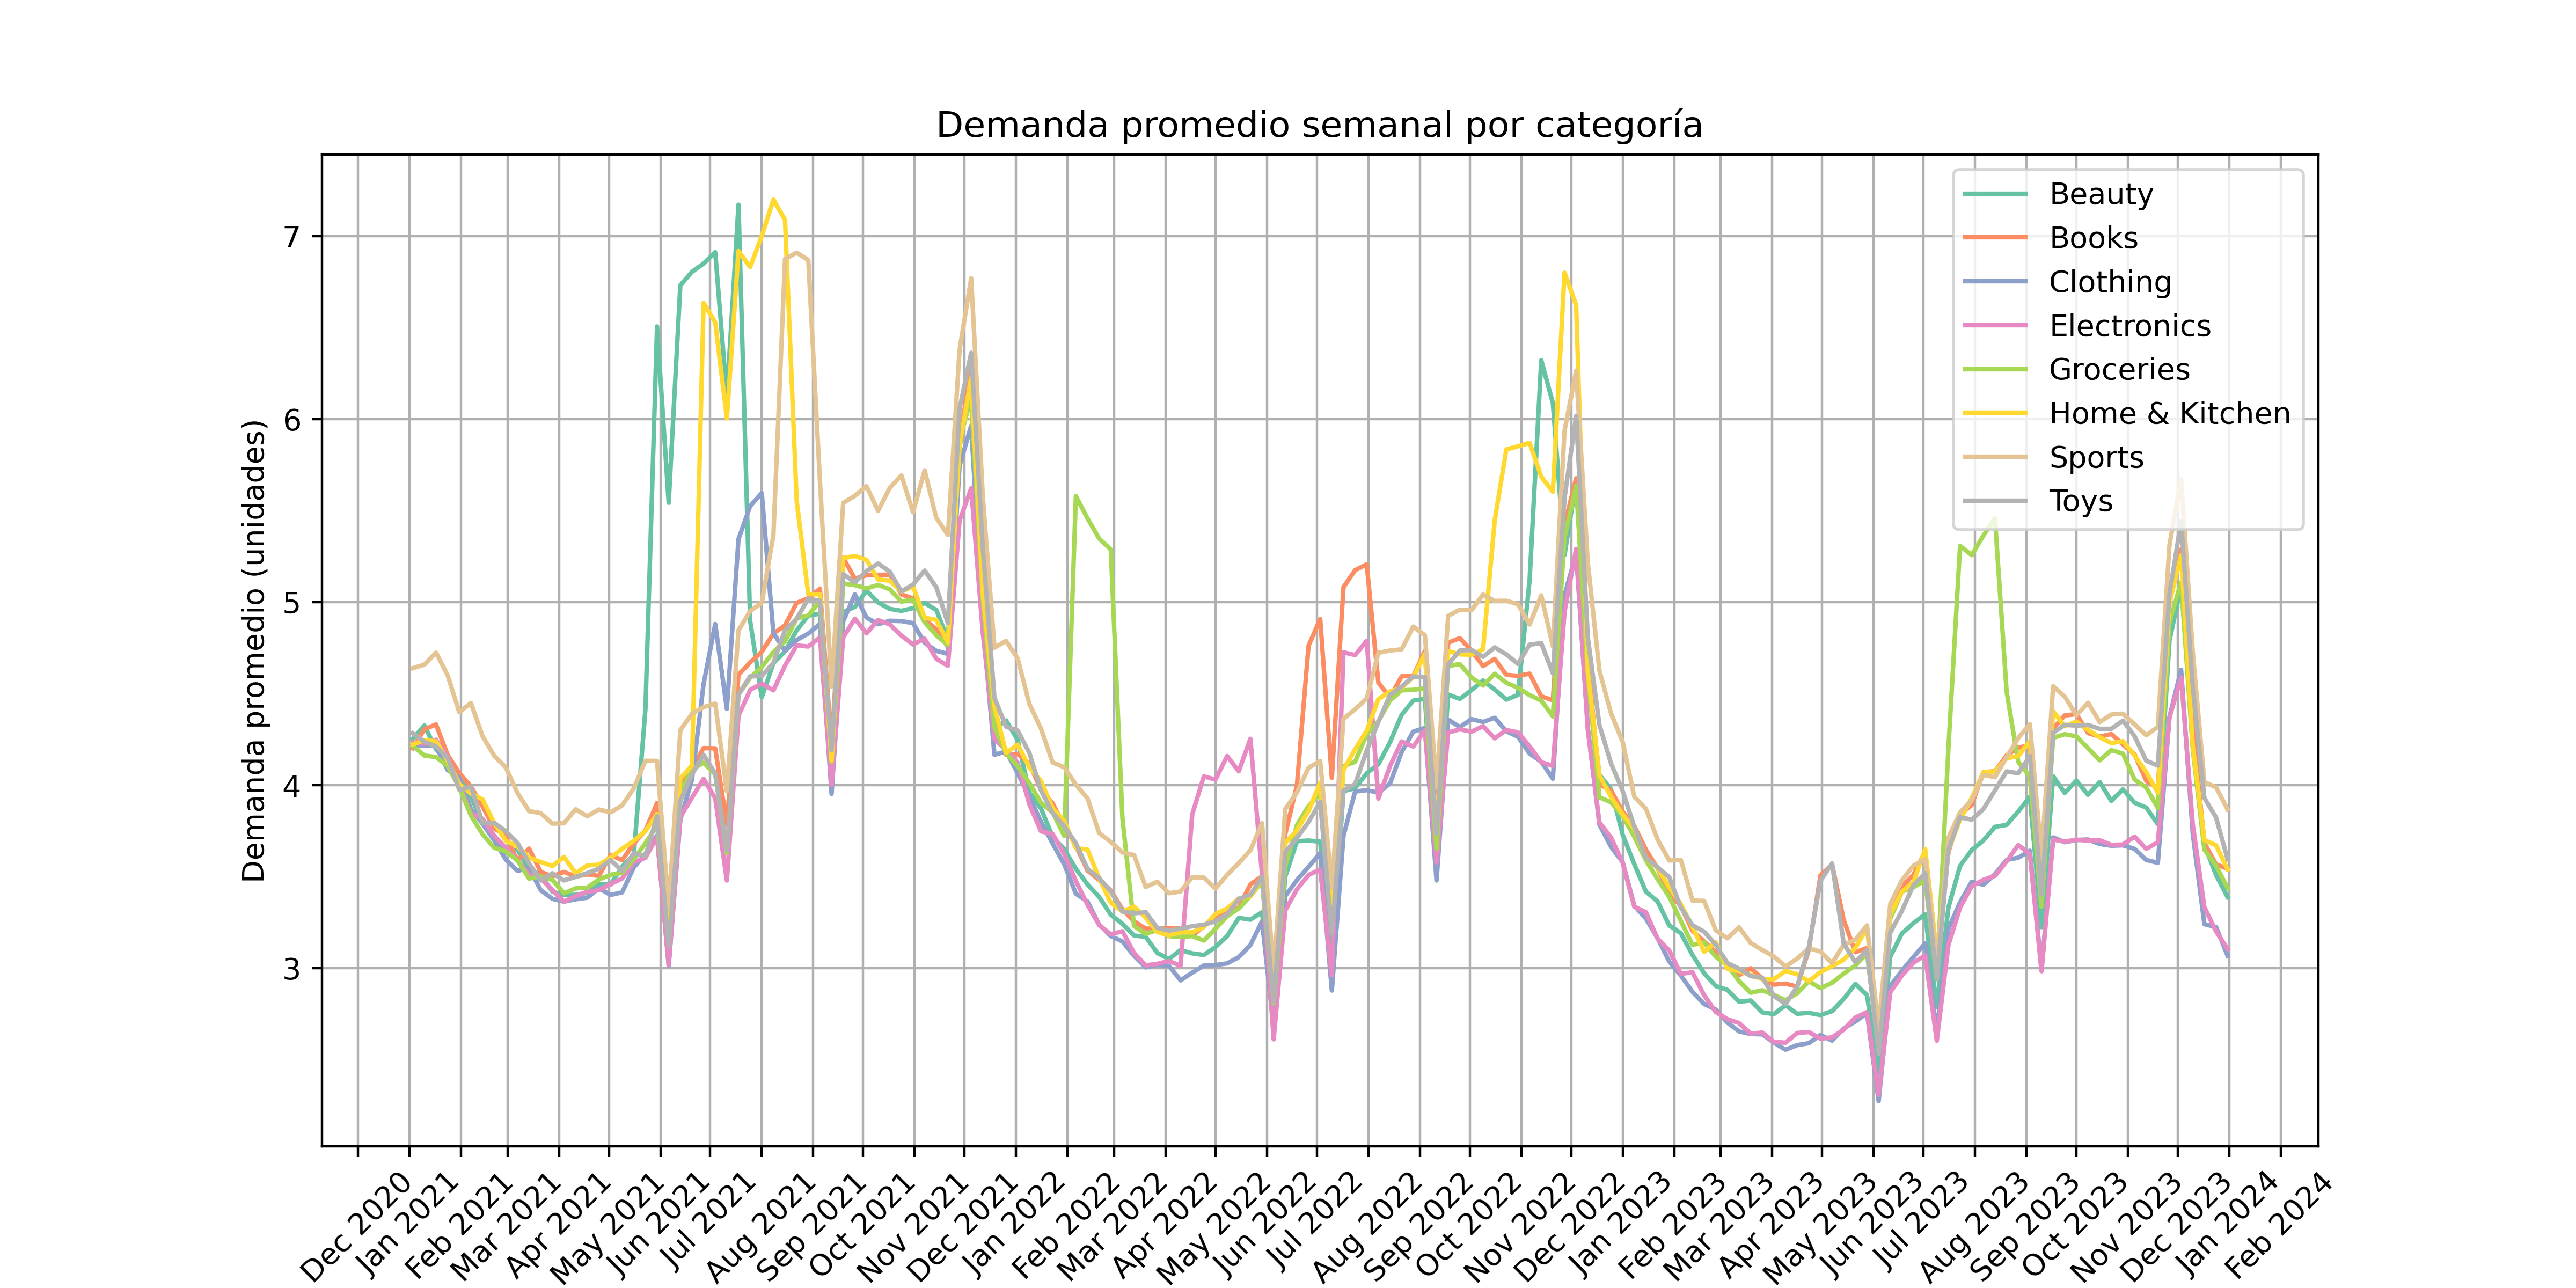
\includegraphics[width=1.2\textwidth]{graficos/demanda_promedio_semanal_por_categoria.png}%
    }
\end{center}

Al comparar este último gráfico con el de las ganancias totales, se pueden observar 3 comportamientos similares: 
\begin{itemize}
    \item A nivel global, hay una reducción gradual de las ganancias y la demanda 
    \item En cada año, en general hay un incremento a medida que transcurre el año y un descenso a principios de cada año.
    \item En Mayo, Junio y Agosto hay caídas abruptas, mientras que en Diciembre hay un incremento sustancial, seguramente debido a las festividades.
\end{itemize}

\section{Análisis Técnico}

\section{Consideraciones Finales}

\end{document}
